\documentclass[journal,12pt,onecolumn]{IEEEtran}
\usepackage{cite}
\usepackage{amsmath,amssymb,amsfonts,amsthm}
\usepackage{algorithmic}
\usepackage{graphicx}
\usepackage{textcomp}
\usepackage{xcolor}
\usepackage{txfonts}
\usepackage{listings}
\usepackage{circuitikz}
\usepackage{enumitem}
\usepackage{mathtools}
\usepackage{gensymb}
\usepackage{comment}
\usepackage[breaklinks=true]{hyperref}
\usepackage{tkz-euclide} 
\usepackage{gvv}                                        
\usepackage[latin1]{inputenc}                                
\usepackage{color}                                            
\usepackage{array}                                            
\usepackage{longtable}                                       
\usepackage{calc}                                             
\usepackage{multirow}                                         
\usepackage{hhline}                                           
\usepackage{ifthen}                                           
\usepackage{lscape}
\usepackage{tabularx}
\usepackage{array}
\usepackage{float}
\usepackage{multicol}
\usepackage{caption}
\usetikzlibrary{patterns}

\newtheorem{theorem}{Theorem}[section]
\newtheorem{problem}{Problem}
\newtheorem{proposition}{Proposition}[section]
\newtheorem{lemma}{Lemma}[section]
\newtheorem{corollary}[theorem]{Corollary}
\newtheorem{example}{Example}[section]
\newtheorem{definition}[problem]{Definition}
\newcommand{\BEQA}{\begin{eqnarray}}
\newcommand{\EEQA}{\end{eqnarray}}
\newcommand{\define}{\stackrel{\triangle}{=}}
\theoremstyle{remark}
\newtheorem{rem}{Remark}

% Marks the beginning of the document
\begin{document}
\bibliographystyle{IEEEtran}
\vspace{3cm}

\title{Assignment 6}
\author{DESABOINA SRI SATHWIK-AI24BTECH11007}
\maketitle
% Removed \newpage to avoid a blank first page
\bigskip

\section*{GATE-2008:ME}

\begin{enumerate}
    \item
	A set of $5$ jobs is to be processed on a single machine. The processing time (in days) is given in the table below. The holding cost for each job is Rs.$K$ per day.\\
		\begin{tabular}[12pt]{ |c| c| c|}
    \hline
    \textbf{S.No} & \textbf{variables used}&\textbf{description}\\ 
    \hline
	$1$ & \textit{t} & a variable which takes the real values in the range $(-1,1)$\\
    \hline
	$2$ & \textit{a} & it is a fixed real number \\
    \hline
	$3$ & $\vec{A(t)}$ & it is a transformation matrix of parameter t\\
    \hline
	$4$ & $\vec{v(t)}$ & it represent the parameter t and allows to define x and y \\
    \hline
	$5$ & $\vec{p(t)}$ & a point with coordinates x and y. \\
    \hline
    \end{tabular}

		A schedule that minimizes the total inventory cost is 

		\hfill{(GATE-ME:2008)}
		\begin{multicols}{2}
			\begin{enumerate}
				\item T-S-Q-R-P
				\item P-R-S-Q-T
				\item T-R-S-Q-P
				\item P-Q-R-S-T
			\end{enumerate}
		\end{multicols}

    \item
        For generating a Coon's surface we require

		\hfill{(GATE-ME:2008)}
        \begin{enumerate}
            
            \item a set of grid points on the surface
            \item a set of grid control points
            \item four bounding curves defining the surface
            \item two bounding curves and a set of grid control points
        \end{enumerate}
    \item
        Internal gear cutting operation can be performed by

        \hfill{(GATE-ME:2008)}
        \begin{enumerate}
            \item milling
            \item shaping with rack cutter
            \item shaping with pinion cutter
            \item hobbing
        \end{enumerate}

 \item
        Consider the shaded triangular region $P$ shown in the figure. What is $\iint\limits_P xydxdy$?
        \vspace{0.2cm}
		\begin{center}
        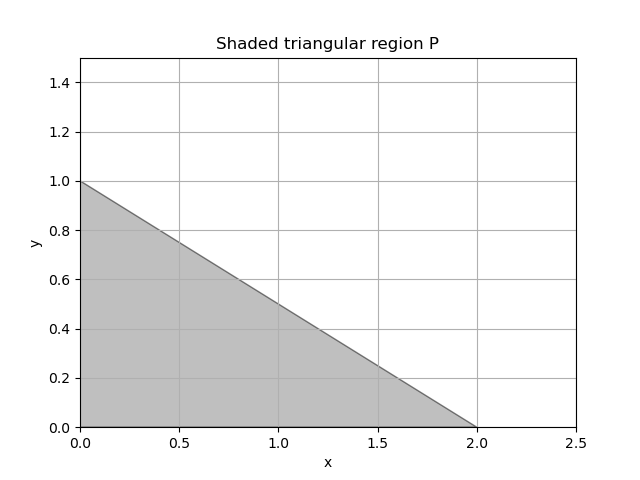
\includegraphics[width=0.4\textwidth]{figs/graph.png}
        \captionof{figure}{}
		\end{center}
        \vspace{0.2cm}

        \hfill{(GATE-ME:2008)}
        \begin{multicols}{4}
            \begin{enumerate}
                \item $\frac{1}{6}$
                \item $\frac{2}{9}$
                \item $\frac{7}{16}$
                \item $1$
            \end{enumerate}
        \end{multicols}
    
    \item 
        The directional derivative of the scalar function $f(x,y,z) = x^2 + 2y^2 + z$ at the point $P = (1,1,2)$ in the direction of the vector $\vec{a} = 3\hat{i} - 4\hat{j}$ is

        \hfill{(GATE-ME:2008)}
        \begin{multicols}{4}
            \begin{enumerate}
                \item $-4$
                \item $-2$
                \item $-1$
                \item $1$\\
            \end{enumerate}
        \end{multicols}

    \item
        For what value of $a$, if any, will the following system of equations in $x, y, z$ have a solution?
              
		\begin{align}
			2x + 3y &= 4 \\
			x + y + z &= 4 \\
			x + 2y - z &= a
                 \end{align}
               
        \hfill{(GATE-ME:2008)}
        \begin{multicols}{2}
            \begin{enumerate}
                \item Any real number
                \item $0$
                \item $1$
                \item There is no such value
            \end{enumerate}
        \end{multicols}
    
    \item
        Which of the following integrals is unbounded?

        \hfill{(GATE-ME:2008)}
        \begin{multicols}{2}
            \begin{enumerate}
                \item $\int_0^{\pi/4} \tan x \, dx$
                \item $\int_0^1 \frac{1}{x^2+1} \, dx$
                \item $\int_0^1 xe^{-x^2} \, dx$
                \item $\int_0^1 \frac{1}{1-x} \, dx$\\
            \end{enumerate}
        \end{multicols}

    \item
        The integral $\oint f(z) dz$ evaluated around the unit circle on the complex plane for $f(z) = \frac{\cos z}{z}$ is
       
       \hfill{(GATE-ME:2008)}
        \begin{multicols}{4}
            \begin{enumerate}
                \item $2\pi i$
                \item $4\pi i$
                \item $-2\pi i$
                \item $0$
            \end{enumerate}
        \end{multicols}
    
    \item
        The length of the curve $y = \frac{2}{3}x^{3/2}$ between $x=0$ and $x=1$ is

        \hfill{(GATE-ME:2008)}
        \begin{multicols}{4}
            \begin{enumerate}
                \item $0.27$
                \item $0.67$
                \item $1$
                \item $1.22$
            \end{enumerate}
        \end{multicols}
    
    \item
	The eigenvectors of the matrix \[\myvec
{1 & 2 \\ 0 & 2} \] are written in the form $\myvec{1\\a}$ and $\myvec{1\\b}.$ What is $a + b$?

        \hfill{(GATE-ME:2008)}
        \begin{multicols}{4}
            \begin{enumerate}
                \item $0$
                \item $\frac{1}{2}$
                \item $1$
                \item $2$
            \end{enumerate}
        \end{multicols}
                                  
    \item 
	Let $f = x^y$. What is $\frac{\partial^2 f}{\partial x \partial y}$ at $x = 2$, $y = 1$?

	 \hfill{(GATE-ME:2008)}

    \begin{multicols}{4}
        \begin{enumerate}
            \item 0
            \item ln 2
            \item 1
            \item $\frac{1}{\ln 2}$
        \end{enumerate}
    \end{multicols}

    \item 
	    It is given that $y^{\prime \prime} + 2y^\prime + y = 0, y(0) = 0, y(1) = 0$. What is $y(0.5)$?

	     \hfill{(GATE-ME:2008)}

    \begin{multicols}{4}
        \begin{enumerate}
            \item 0
            \item 0.17
            \item 0.62
            \item 1.13
        \end{enumerate}
    \end{multicols}

    \item The strain energy stored in the beam with flexural rigidity $EI$ and loaded as shown in the figure is
	    \begin{center}
	    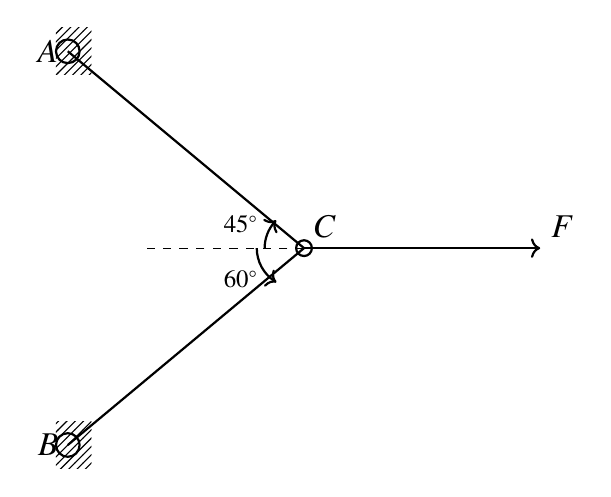
\begin{tikzpicture}
    % Define points with A and B further left and spaced vertically
    \coordinate (A) at (-3,2.5);
    \coordinate (B) at (-3,-2.5);
    \coordinate (C) at (0,0);
    \coordinate (F) at (3,0);

    % Draw fixed supports at A and B
    \fill[pattern=north east lines] (-3.15,2.8) rectangle (-2.7,2.2);
    \fill[pattern=north east lines] (-3.15,-2.2) rectangle (-2.7,-2.8);
    
    % Draw circles at supports
    \draw[thick] (A) circle(0.15);
    \draw[thick] (B) circle(0.15);
    \draw[thick] (C) circle(0.1);

    % Draw the rods AC and BC
    \draw[thick] (A) -- (C);
    \draw[thick] (B) -- (C);

    % Draw force arrow at C and label at the end
    \draw[thick, ->] (C) -- (F) node[above right] {\large $F$};

    % Draw a dashed line from C to the left
    \draw[dashed] (C) -- ++(-2,0);

    % Draw angle arcs and labels in correct positions
    \draw[thick, ->] (-0.5,0) arc[start angle=180, end angle=135, radius=0.5];
    \node at (-0.8,0.3) {\small $45^\circ$};
    
    \draw[thick, ->] (-0.6,0) arc[start angle=180, end angle=240, radius=0.5];
    \node at (-0.8,-0.4) {\small $60^\circ$};

    % Label points A, B, and C
    \node[left] at (A) {\large $A$};
    \node[left] at (B) {\large $B$};
    \node[above right] at (C) {\large $C$};

\end{tikzpicture}

	    \end{center}
 
 \hfill{(GATE-ME:2008)}
 \begin{multicols}{2}
	 \begin{enumerate}
	    \item $\frac{P^2 L^3}{3EI}$
            \item $\frac{2P^2 L^3}{3EI}$
            \item $\frac{4P^2 L^3}{3EI}$
            \item $\frac{8P^2 L^3}{3EI}$
	    
        \end{enumerate}
    \end{multicols}

    \item For the component loaded with a force $F$ as shown in the figure, the axial stress at the corner point $P$ is
	    \begin{center}
	    \begin{tikzpicture}
    % Draw the x and y axes
    \draw[->] (-1.5, 0) -- (1.5, 0) node[right] {$x$};
    \draw[->] (0, -1.5) -- (0, 1.5) node[above] {$y$};
    
    % Draw the optic axis at 135° angle
    \draw[dashed, ->] (1.2, -1.2) -- (-1.2, 1.2);
    \node at (-2, 1) {Optic axis};

    
    % Draw the 135° angle arc
    \draw[->] (0.5, 0) arc[start angle=0, end angle=135, radius=0.5];
    \node at (0.8, 0.3) {$135^\circ$};
\end{tikzpicture}


	    \end{center}

	     \hfill{(GATE-ME:2008)}

       \begin{multicols}{4}
        \begin{enumerate}
            \item $\frac{F(3L-b)}{4b^3}$
            \item $\frac{F(3L+b)}{4b^3}$
            \item $\frac{F(3L-4b)}{4b^3}$
            \item $\frac{F(3L-2b)}{4b^3}$
        \end{enumerate}
    \end{multicols}

    \item A solid circular shaft of diameter 100 mm is subjected to an axial stress of 50 MPa. It is further subjected to a torque of 10 kNm. The maximum principal stress experienced on the shaft is closest to

	     \hfill{(GATE-ME:2008)}

    \begin{multicols}{4}
        \begin{enumerate}
            \item 41 MPa
            \item 82 MPa
            \item 164 MPa
            \item 204 MPa
        \end{enumerate}
    \end{multicols}

    \item A circular disk of radius $R$ rolls without slipping at a velocity $v$. The magnitude of the velocity at point $P$ is\\
	    \begin{center}
	    \begin{circuitikz}
    % Voltage source Vin
    \draw (0,0) to[open,v^=$V_{in}$] (0,3);
    \draw (0,3) -- (1,3) to[R=$R$] (3,3) to[short] (4,3);
    \draw (1,3.5) node[]{$5\ \mathrm{V}$} -- (1,3);
    \draw (1,0) node[]{$0\ \mathrm{V}$} -- (1,0.5);

    % Transistor and resistor network
    \draw (4,3) to[R=$1\ \mathrm{k}\Omega$] (4,1) to[short] (5,1) -- (5,-1) node[ground]{};
    \draw (4,3) -- (6,3) node[npn, anchor=B] (Q1) {};
    \node at (Q1) {Q};

    % Vcc and collector resistor
    \draw (6,5) node[vcc]{$+5\ \mathrm{V}$} to[R=$5\ \mathrm{k}\Omega$] (6,3.5) -- (6,3);

    % Resistor at emitter
    \draw (Q1.E) to[R=$100\ \Omega$] (6,-1) node[ground]{};

    % Output
    \draw (6,3) to[open,v^=$V_{out}$] (8,3);
    \draw (8,3.5) node[]{$5\ \mathrm{V}$};
    \draw (8,0.5) node[]{$0\ \mathrm{V}$};

    % Negative voltage
    \draw (4,1) -- (3,1) node[ground] {};
    \draw (3.5,0.5) node[]{$-12\ \mathrm{V}$};

\end{circuitikz}

	    \end{center}

	     \hfill{(GATE-ME:2008)}

       \begin{multicols}{4}
        \begin{enumerate}
            \item $\frac{\sqrt{3}}{v}$
            \item $\frac{\sqrt{3} v}{2}$
            \item $\frac{v}{2}$
            \item $v \sqrt{3}$
        \end{enumerate}
    \end{multicols}

    \item Consider a truss PQR loaded at $P$ with a force $F$ as shown in the figure. The tension in the member $QR$ is\\
	    \begin{center}
	    \begin{tikzpicture}

% Define points
\coordinate (Q) at (0,0);
\coordinate (R) at (6,0);
\coordinate (P) at (3,3);

% Draw the truss members
\draw[thick] (Q) -- (P) -- (R);
\draw[thick] (Q) -- (R);

% Draw the force F
\draw[thick,<-] (P) -- +(0,2) node[above] {$F$};

% Draw support at Q (hinged)
\draw[thick] (Q) -- +(-0.5,-0.5);
\draw[thick] (Q) -- +(0.5,-0.5);
\draw[thick] (Q) -- +(0,-0.7);

% Draw support at R (roller)
\draw[thick] (R) -- +(0,-0.5);
\draw[thick] (R) -- +(0.5,-0.5);
\draw[thick] (R) -- +(0,-0.7);
\draw[thick] (R) -- +(-0.5,-0.5);

% Add angle markers
\draw[thick] (0.5,0) arc[start angle=0,end angle=45,radius=0.5];
\node at (0.8,0.25) {$45^\circ$};

\draw[thick] (5.5,0) arc[start angle=180,end angle=150,radius=0.8];
\node at (5,0.25) {$30^\circ$};

% Label points
\node at (Q) [left] {$Q$};
\node at (R) [right] {$R$};
\node at (P) [above left] {$P$};

\end{tikzpicture}

	    \end{center}

	     \hfill{(GTE-ME:2008)}

       \begin{multicols}{4}
        \begin{enumerate}
            \item $0.5F$
            \item $0.63F$
            \item $0.73F$
            \item $0.87F$
        \end{enumerate}
    \end{multicols}


\end{enumerate}
\end{document}

